\documentclass{beamer}

% Metropolis theme (modern, minimal)
\usetheme{metropolis}
\usepackage{appendixnumberbeamer}

\usepackage{xcolor}
\usepackage{mathrsfs}
\usepackage{amsmath}
\usepackage{amssymb}
\usepackage{booktabs}
\usepackage{hyperref}
\pdfstringdefDisableCommands{\def\translate#1{#1}}
\usepackage{animate}
\usepackage{caption}
\usepackage{graphicx}
\usepackage{subcaption}
\usepackage{tikz}
\usepackage{multirow}
\usetikzlibrary{arrows.meta, positioning, shapes.geometric, shadows}
\usepackage{tcolorbox}
\tcbuselibrary{skins, breakable}
\captionsetup{font=tiny}
\graphicspath{{../figures/}}

\usepackage[
    backend=biber,
    style=alphabetic,
    sorting=ynt
]{biblatex}
\addbibresource{bibliography.bib}

% Colour palette
\definecolor{CSred}{RGB}{160,32,60}
\definecolor{CSgrey}{RGB}{136,121,150}
\definecolor{CSlight}{RGB}{245,240,248}
\definecolor{alertorange}{RGB}{200,80,0}
\definecolor{metrobg}{RGB}{255,255,255}
\definecolor{greenok}{RGB}{34,120,60}

% Metropolis overrides
\setbeamercolor{normal text}{fg=black!85, bg=metrobg}
\setbeamercolor{frametitle}{bg=CSred, fg=white}
\setbeamercolor{title separator}{fg=CSred}
\setbeamercolor{progress bar}{fg=CSred, bg=CSgrey!40}
\setbeamercolor{alerted text}{fg=CSred}
\setbeamercolor{block title}{bg=CSred, fg=white}
\setbeamercolor{block body}{bg=CSlight}
\setbeamercolor{block title alerted}{bg=alertorange, fg=white}
\setbeamercolor{block body alerted}{bg=orange!7}
\metroset{progressbar=frametitle, sectionpage=none, numbering=fraction}
\setbeamerfont{frametitle}{series=\bfseries, size=\normalsize}

% tcolorbox styles
\tcbset{
  keybox/.style={
    colback=CSlight, colframe=CSred, fonttitle=\bfseries\small,
    boxrule=0.8pt, arc=3pt, left=5pt, right=5pt, top=4pt, bottom=4pt
  },
  warnbox/.style={
    colback=orange!7, colframe=alertorange, fonttitle=\bfseries\small,
    boxrule=0.8pt, arc=3pt, left=5pt, right=5pt, top=4pt, bottom=4pt
  },
  stressbox/.style={
    colback=CSlight, colframe=CSgrey, fonttitle=\bfseries\footnotesize,
    boxrule=0.8pt, arc=4pt, left=4pt, right=4pt, top=3pt, bottom=3pt
  },
  resultbox/.style={
    colback=green!5, colframe=greenok, fonttitle=\bfseries\small,
    boxrule=0.8pt, arc=3pt, left=5pt, right=5pt, top=4pt, bottom=4pt
  }
}

% Appendix toggle (suppress TOC slides in the appendix)
\newif\ifinappendix
\inappendixfalse
\let\origappendix\appendix
\renewcommand{\appendix}{\origappendix\inappendixtrue}

% Auto-insert outline frame at each section transition
\AtBeginSection[]{%
  \ifinappendix\else
  \begin{frame}{Outline}
        \tableofcontents[currentsection,hideothersubsections]
  \end{frame}
  \fi
}

% tcolorbox styles
\tcbset{
  keybox/.style={
    colback=CSlight, colframe=CSred, fonttitle=\bfseries\small,
    boxrule=0.8pt, arc=3pt, left=5pt, right=5pt, top=4pt, bottom=4pt
  },
  warnbox/.style={
    colback=orange!7, colframe=alertorange, fonttitle=\bfseries\small,
    boxrule=0.8pt, arc=3pt, left=5pt, right=5pt, top=4pt, bottom=4pt
  },
  resultbox/.style={
    colback=green!5, colframe=greenok, fonttitle=\bfseries\small,
    boxrule=0.8pt, arc=3pt, left=5pt, right=5pt, top=4pt, bottom=4pt
  }
}

\setbeamertemplate{note page}[plain]

\title{Probabilistic Detection of Market Manipulation}
\subtitle{MDS Project - Final Presentation}
\author[Adonis Jamal \and Jean Martini]{Adonis~Jamal \and Jean Martini\\Supervisor: Damien Challet\\Tutor: Lionel Gabet}
\institute{CentraleSupélec, MICS Laboratory}
\date{April 14, 2026}

\titlegraphic{%
    \hfill
    
\includegraphics[height=0.8cm]{img/logo_cs}
    \hspace{0.4cm}
    
\includegraphics[height=0.8cm]{img/logoMICS.png}
}

\begin{document}

% ======================================================================
% SLIDE 1: TITLE
% ======================================================================
\frame{\titlepage}

% ======================================================================
% SLIDE 2: OUTLINE
% ======================================================================
\begin{frame}{Outline}
    \tableofcontents[hideallsubsections]
\end{frame}


% ######################################################################
% SECTION 1: PROBLEM AND MOTIVATION
% ######################################################################
\section{Introduction and Methodology}
\subsection{Problem and Motivation}

% ======================================================================
% SLIDE 3: LOB AND SPOOFING
% ======================================================================
\begin{frame}{Spoofing in the Limit Order Book}
    \begin{tcolorbox}[keybox, title=Mechanism]
        \begin{itemize}
            \item Non-bona fide orders placed to create false supply/demand pressure
            \item Mid-price shifts towards the manipulator's genuine order
            \item Spoof orders cancelled once the genuine order is filled
        \end{itemize}
    \end{tcolorbox}
    \begin{tcolorbox}[warnbox, title=Detection Challenges]
        \begin{itemize}
            \item \textbf{Contamination:} training data contains unknown manipulations
            \item \textbf{No ground truth:} no ``manipulated / not manipulated'' labels
            \item \textbf{Non-stationarity:} market regime changes (volatility, liquidity)
        \end{itemize}
    \end{tcolorbox}
    \note{Spoofing is prohibited under EU MAR and the US Dodd-Frank Act, yet detection remains difficult because the same order flow patterns arise from legitimate trading strategies. The absence of labels forces an unsupervised, score-based approach.}
\end{frame}

% ======================================================================
% SLIDE 4: WHY PROBABILISTIC, SCORE-BASED DETECTION
% ======================================================================
\begin{frame}{Why Probabilistic, Score-Based Detection}
    \begin{itemize}
        \item No ground-truth labels exist at the order level in equity markets
        \item Manipulation is a spectrum of intent, not a discrete category
        \item A continuous score allows ranking events by severity and calibrating thresholds to a desired false discovery rate
    \end{itemize}

    \textbf{Research questions:}
    \begin{itemize}
        \item Can unsupervised models detect anomalous order flow without labels?
        \item Do different models agree on the same discriminative features?
        \item Can spoofing profitability be estimated directly from model predictions?
        \item Do detection patterns remain stable across years?
    \end{itemize}
\end{frame}


% ######################################################################
% SECTION 2: METHODOLOGY OVERVIEW
% ######################################################################
\subsection{Methodology Overview}

% ======================================================================
% SLIDE 5: PIPELINE OVERVIEW (TikZ)
% ======================================================================
\begin{frame}{Detection Pipeline}
\centering
\resizebox{0.95\textwidth}{!}{%
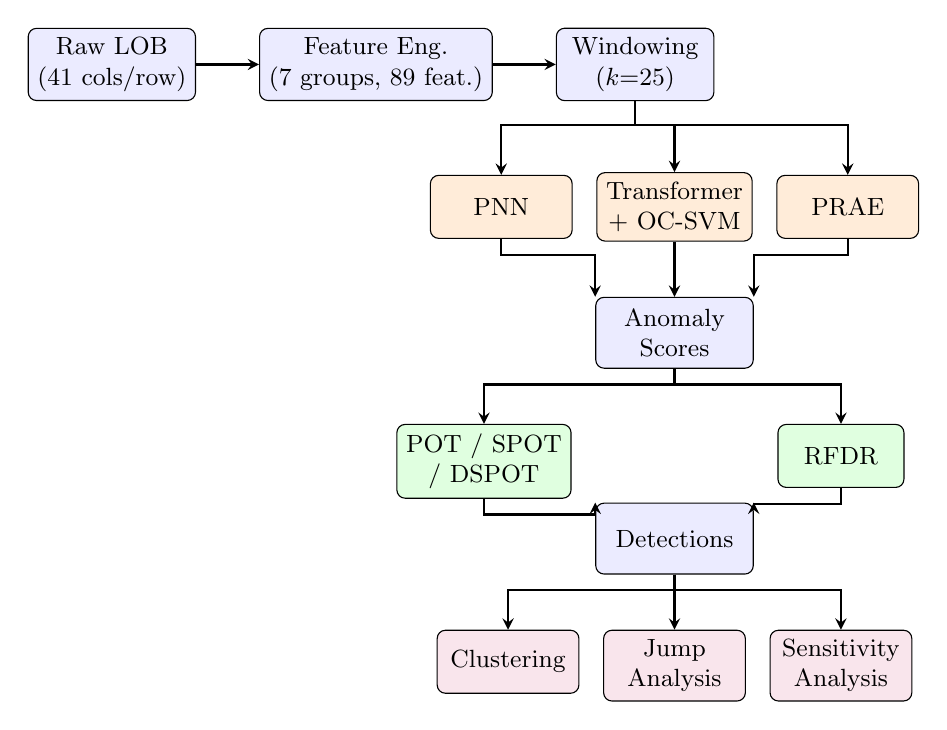
\begin{tikzpicture}[
  node distance=0.6cm and 0.8cm,
  stage/.style={rectangle, draw, rounded corners=3pt, minimum height=0.9cm, minimum width=2cm,
                align=center, font=\small, fill=blue!8},
  model/.style={rectangle, draw, rounded corners=3pt, minimum height=0.8cm, minimum width=1.8cm,
                align=center, font=\small, fill=orange!15},
  threshold/.style={rectangle, draw, rounded corners=3pt, minimum height=0.8cm, minimum width=1.6cm,
                    align=center, font=\small, fill=green!12},
  posthoc/.style={rectangle, draw, rounded corners=3pt, minimum height=0.8cm, minimum width=1.8cm,
                  align=center, font=\small, fill=purple!10},
  arr/.style={->, thick, >=stealth},
]
  \node[stage] (raw) {Raw LOB\\(41 cols/row)};
  \node[stage, right=of raw] (feat) {Feature Eng.\\(7 groups, 89 feat.)};
  \node[stage, right=of feat] (win) {Windowing\\($k{=}25$)};
  \node[model, below right=0.9cm and -1.5cm of win] (tfocsvm) {Transformer\\+ OC-SVM};
  \node[model, left=0.3cm of tfocsvm] (pnn) {PNN};
  \node[model, right=0.3cm of tfocsvm] (prae) {PRAE};
  \node[stage, below=0.7cm of tfocsvm] (scores) {Anomaly\\Scores};
  \node[threshold, below left=0.7cm and 0.3cm of scores] (evt) {POT / SPOT\\/ DSPOT};
  \node[threshold, below right=0.7cm and 0.3cm of scores] (rfdr) {RFDR};
  \node[stage, below=0.7cm of scores, yshift=-1.0cm] (det) {Detections};
  \node[posthoc, below left=0.7cm and 0.2cm of det] (clust) {Clustering};
  \node[posthoc, below=0.7cm of det] (jump) {Jump\\Analysis};
  \node[posthoc, below right=0.7cm and 0.2cm of det] (ig) {Sensitivity\\Analysis};
  \draw[arr] (raw) -- (feat);
  \draw[arr] (feat) -- (win);
  \draw[arr] (win.south) -- ++(0,-0.3) -| (pnn.north);
  \draw[arr] (win.south) -- ++(0,-0.3) -| (tfocsvm.north);
  \draw[arr] (win.south) -- ++(0,-0.3) -| (prae.north);
  \draw[arr] (pnn.south) -- ++(0,-0.2) -| (scores.north west);
  \draw[arr] (tfocsvm.south) -- (scores.north);
  \draw[arr] (prae.south) -- ++(0,-0.2) -| (scores.north east);
  \draw[arr] (scores.south) -- ++(0,-0.2) -| (evt.north);
  \draw[arr] (scores.south) -- ++(0,-0.2) -| (rfdr.north);
  \draw[arr] (evt.south) -- ++(0,-0.2) -| (det.north west);
  \draw[arr] (rfdr.south) -- ++(0,-0.2) -| (det.north east);
  \draw[arr] (det.south) -- ++(0,-0.2) -| (clust.north);
  \draw[arr] (det.south) -- (jump.north);
  \draw[arr] (det.south) -- ++(0,-0.2) -| (ig.north);
\end{tikzpicture}%
}
    \note{The pipeline transforms 41-column LOB snapshots into 89 engineered features, windows them into sequences of length 25, and scores each window with three complementary models. Threshold methods convert scores to binary detections for post-hoc analysis.}
\end{frame}

% ======================================================================
% SLIDE 6: FEATURE ENGINEERING
% ======================================================================
\begin{frame}{Feature Engineering: 89 Features in 7 Groups}
    \begin{table}[h]
    \centering
    \footnotesize
    \begin{tabular}{lrl}
    \toprule
    \textbf{Group} & \textbf{Count} & \textbf{Key quantities} \\
    \midrule
    Imbalance          & 5  & L1/L5 imbalance, 3 weighted schemes \cite{tao_2020} \\
    Price dynamics     & 13 & Mid-price, spread, log return, depth ratio \\
    Elasticity         & 4  & Sweep cost ($Q{=}1000$), book slope ($D{=}5$) \\
    Volatility         & 6  & Rolling $\sigma$ ($W{=}50,100$), price range, $\Delta t$ \\
    Event flow         & 18 & Cancel/trade size \& rapidity \cite{poutre_2024} \\
    Hawkes memory      & 38 & Spatial + temporal decay, $4\eta \times 3\beta$ \cite{fabre_2025} \\
    OFI                & 5  & Multi-level order flow imbalance (L1 to L5) \\
    \midrule
    \textbf{Total}     & \textbf{89} & ${\sim}7{\times}$ larger than Poutr{\'e} et al.\ (${\sim}13$) \\
    \bottomrule
    \end{tabular}
    \end{table}
    \begin{itemize}
        \item Preprocess: inf/NaN fix, 3,000-row warmup trim. Clip features: $[0.1\%, 99.9\%]$ quantiles
        \item Scale: Empirical Box-Cox then z-score, fitted on day~1 only
    \end{itemize}
    \note{The feature library integrates contributions from three reference papers. Hawkes memory features capture self-exciting order flow patterns with spatial decay, absent from Poutr\'e et al.'s Level-1 feature set.}
\end{frame}

% ======================================================================
% SLIDE 7: MODEL 1: TRANSFORMER + OC-SVM
% ======================================================================
\begin{frame}{Model 1: Transformer Bottleneck AE + OC-SVM \cite{poutre_2024}}
    \begin{tcolorbox}[keybox, title=Why this model]
        \begin{itemize}
            \item Self-attention captures long-range LOB dependencies (price levels, event sequences)
            \item Bottleneck: 2,225 dimensions to 128 latent features
            \item Latent OC-SVM beats raw reconstruction error \cite{poutre_2024}. Normal data and anomalies more separable in latent space.
            \item \textbf{Limitation:} signed distance, uncalibrated probability
        \end{itemize}
    \end{tcolorbox}
    \begin{tcolorbox}[keybox, title=Inference]
        AE trains end-to-end for reconstruction. At inference, decoder discarded and encoder outputs latent vectors for OC-SVM. Dissimilarity score $d_t$ is flagged when $d_t \geq \tau$.
    \end{tcolorbox}
\end{frame}

% ======================================================================
% SLIDE 8: MODEL 2: PNN
% ======================================================================
\begin{frame}{Model 2: Probabilistic Neural Network \cite{fabre_2025}}
    \begin{tcolorbox}[keybox, title=Why this model]
        \begin{itemize}
            \item Predicts full conditional next-move distribution
            \item Outputs likelihood score and spoofing gain
            \item Gain gives direct economic interpretability: Expected profit
            \item \textbf{Limitation:} strategy-model dependence can miss patterns
        \end{itemize}
    \end{tcolorbox}
    \begin{tcolorbox}[keybox, title=Anomaly Score]
        Spoofing gain $G_t = \mathbb{E}[C_{\text{normal}}] - \mathbb{E}[C_{\text{spoof}}]$; flagged if $G_t > 0$ (spoofing profitable). Thresholding is implicit: the economic framework supplies it.
    \end{tcolorbox}
    \note{Architecture details (hidden dimension, skew-normal parameterisation, loss function) are in the appendix. The PNN is Markovian: it uses only the last time step of each window. Spoofing gain parameters: $Q{=}4500$, $q{=}100$, $\delta_b{=}0.01$, maker fee 0, taker fee 0.0008 (Euronext Paris large-cap schedule).}
\end{frame}

% ======================================================================
% SLIDE 9: MODEL 3: PRAE
% ======================================================================
\begin{frame}{Model 3: Probabilistic Robust Autoencoder \cite{lindenbaum2022prae}}
    \begin{tcolorbox}[keybox, title=Why this model]
        \begin{itemize}
            \item Per-sample gate downweights suspected anomalies
            \item Robustness under unknown contamination rates
            \item \textbf{Limitation:} reduces to standard autoencoder if gates collapse
        \end{itemize}
    \end{tcolorbox}
    \begin{tcolorbox}[keybox, title=Anomaly Score]
        Reconstruction error $s_t = \|S_t - \hat{S}_t\|^2$; higher implies stronger anomaly
    \end{tcolorbox}
    \note{Architecture details (gate parameterisation, loss function, $\lambda$ tuning) are in the appendix. The PRAE shares the same Transformer backbone as TF-OCSVM. The gating mechanism was designed to downweight contaminated training samples, but in practice the $\ell_1$ regularisation weight and noise level were insufficient to force the gate to discriminate.}
\end{frame}

% ======================================================================
% SLIDE 10: THRESHOLDING METHODS
% ======================================================================
\begin{frame}{Anomaly Thresholding: Four Label-Free Methods}
    Two models (TF-OC-SVM, PRAE) produce continuous scores requiring explicit threshold selection.
    \vspace{0.15cm}
    \begin{table}[h]
    \centering
    \footnotesize
    \begin{tabular}{lp{6.5cm}}
    \toprule
    \textbf{Method} & \textbf{Mechanism} \\
    \midrule
    POT  & Batch EVT: fits GPD to exceedances above 98th percentile \\
    SPOT \cite{siffer:hal-01640325} & Streaming EVT: updates GPD parameters as new peaks arrive \\
    DSPOT \cite{siffer:hal-01640325} & Drift-aware SPOT: adds moving-average correction for non-stationarity \\
    RFDR & Rolling Benjamini-Hochberg: controls false discovery rate at $\alpha$ on a sliding window \\
    \bottomrule
    \end{tabular}
    \end{table}
    \begin{itemize}
        \item TF-OCSVM baseline: $\tau_0 = Q_{1-\nu}$ (vs. $F_4$ score \cite{poutre_2024})
        \item PNN threshold: $G_t > 0$
    \end{itemize}
    \note{DSPOT degenerates on PNN bounded scores (flags 99.8\%). RFDR and POT are the most stable label-free methods across all three score streams.}
\end{frame}

% ======================================================================
% SLIDE 11: EXPERIMENTAL SETUP
% ======================================================================
\begin{frame}{Experimental Setup}
    \begin{table}[h]
    \centering
    \footnotesize
    \begin{tabular}{ll}
    \toprule
    \textbf{Parameter} & \textbf{Value} \\
    \midrule
    Instrument         & TOTF.PA (TotalEnergies, Euronext Paris) \\
    Training period 1  & 2015 (13 days) \\
    Training period 2  & 2017 (61 days) \\
    Proximate test ($\mathcal{T}_A$) & 9 days per year \\
    Distal test ($\mathcal{T}_B$)    & 3 days per year \\
    Out-of-sample      & 2010 (261 days), cross-year \\
    Training window    & First hour only (09:00 to 10:00), alternating 5-min blocks \\
    Test window        & Full session (09:00 to 17:30) \\
    Intraday periods   & 4 (first hour, rest of morning, afternoon, US open) \\
    \bottomrule
    \end{tabular}
    \end{table}
    \note{The asymmetry between training (first hour) and testing (full session) is deliberate: it tests whether patterns learned in the opening hour generalise to the rest of the trading day.}
\end{frame}


% ######################################################################
% SECTION 3: MODEL DIAGNOSTICS
% ######################################################################
\section{Experimental Results}
\subsection{Model Diagnostics}

% ======================================================================
% SLIDE 12: TF-OCSVM DIAGNOSTICS
% ======================================================================
\begin{frame}{TF-OCSVM: Latent Representation and Threshold Calibration}
    \begin{columns}[T]
    \begin{column}{0.48\textwidth}
        \centering
        \includegraphics[width=\linewidth]{../figures/diagnostics/tfocsvm_latent_pca_2015.pdf}\\
        {\tiny 2015: first 2 PCs capture 10.2\% variance}
    \end{column}
    \begin{column}{0.48\textwidth}
        \centering
        \includegraphics[width=\linewidth]{../figures/diagnostics/tfocsvm_latent_pca_2017.pdf}\\
        {\tiny 2017: first 2 PCs capture 17.8\% variance}
    \end{column}
    \end{columns}
    
    \begin{itemize}
        \item Dense inlier cluster, peripheral outliers: tighter boundary
        \item 2017 latent structure stronger: 17.8\% vs 10.2\%
        \item Unbounded score: percentile thresholds not equivalent
        \item Reconstruction and dissimilarity nearly orthogonal ($r \approx -0.16$): complementary information
    \end{itemize}
    \note{No dimension collapses to zero variance and the bottleneck capacity is fully utilised. Pairwise kernel values concentrate in $(0, 0.1)$, confirming discriminative $\gamma$ calibration. $\tau_{2015} = -0.019$ (flags 0.21\%); $\tau_{2017} \approx -0.001$ (flags 0.045\%).}
\end{frame}

% ======================================================================
% SLIDE 13: PNN DIAGNOSTICS
% ======================================================================
\begin{frame}{PNN: Predicted Distribution Parameters by Year}
    \begin{columns}[T]
    \begin{column}{0.48\textwidth}
        \centering
        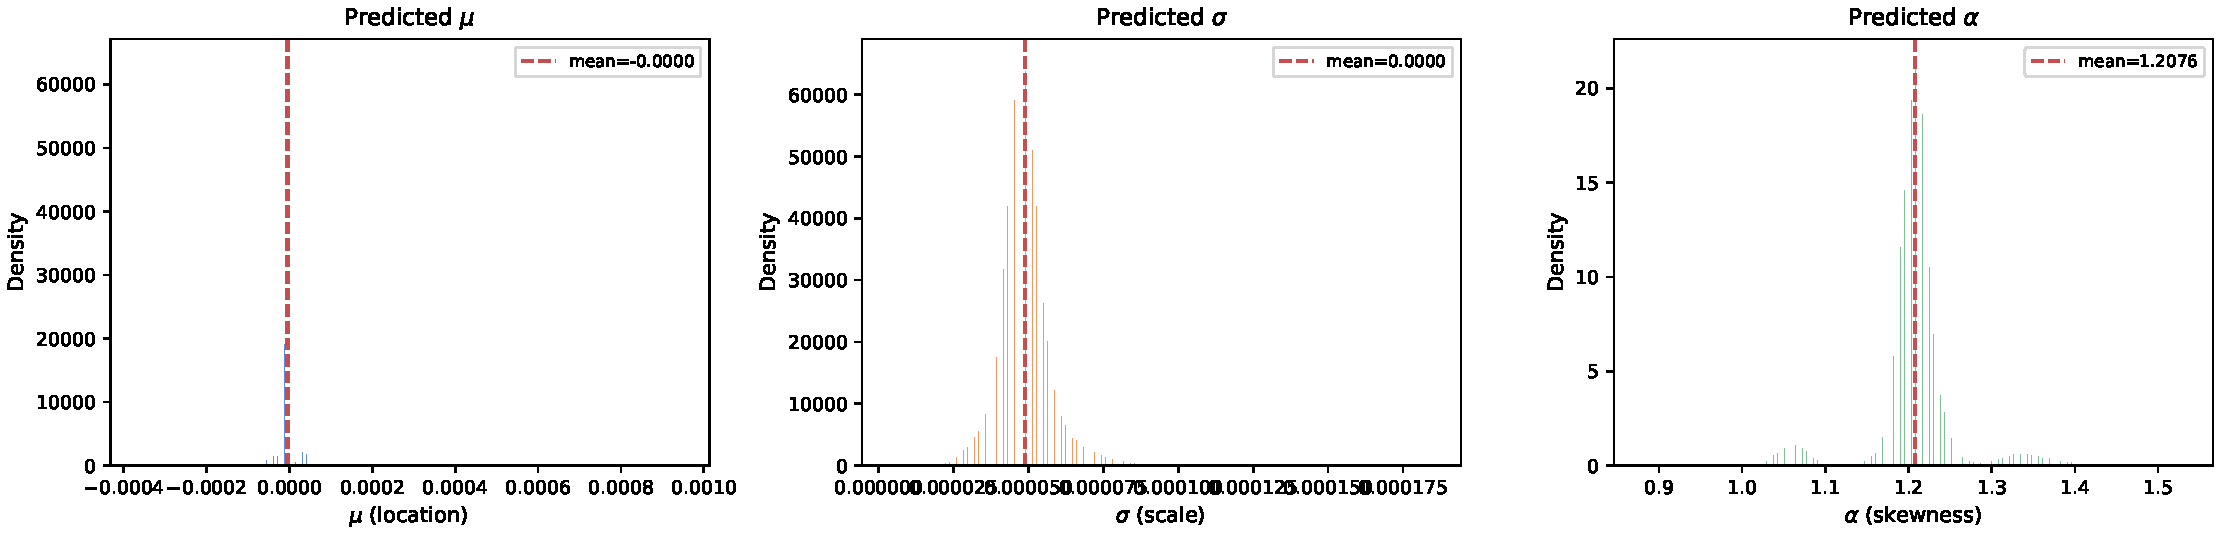
\includegraphics[width=\linewidth]{../figures/diagnostics/pnn_parameters_2015.pdf}\\
        {\tiny 2015: $\bar{\sigma} = 4.9 \times 10^{-5}$, $\bar{\alpha} = +1.21$}
    \end{column}
    \begin{column}{0.48\textwidth}
        \centering
        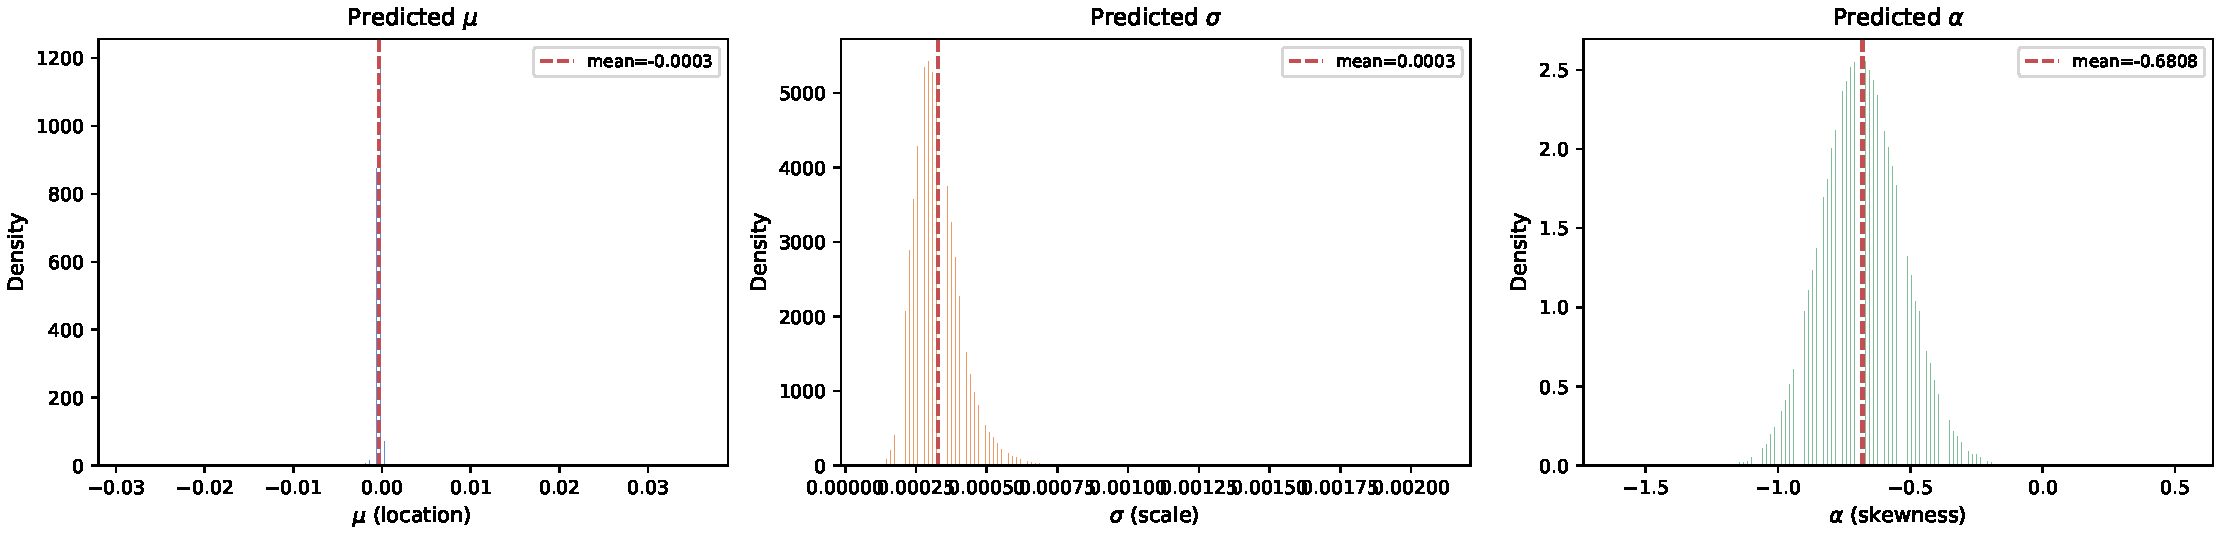
\includegraphics[width=\linewidth]{../figures/diagnostics/pnn_parameters_2017.pdf}\\
        {\tiny 2017: $\bar{\sigma} = 3.3 \times 10^{-4}$, $\bar{\alpha} = -0.68$}
    \end{column}
    \end{columns}
    \vspace{0.2cm}
    \begin{itemize}
        \item 2015 $\sigma$ narrower by factor 6.7: small price deviations appear extreme
        \item Narrow $\sigma$: inflated 2015 anomaly rate
        \item Positive gain alignment on 2017 calibration
        \item Cross-year rates confounded by distributional shift
    \end{itemize}
    \note{The narrow $\sigma$ learned on 2015 data implies overconfidence: the PNN produces positive spoofing gains even for typical price moves. The broader $\sigma$ on 2017 data results in a more conservative flag rate. Skewness sign reversal: positive (2015) vs.\ negative (2017). 99th-percentile NLL: 0.20 (2015) vs.\ 23.0 (2017).}
\end{frame}

% ======================================================================
% SLIDE 14: PRAE DIAGNOSTICS
% ======================================================================
\begin{frame}{PRAE: Gate Collapse and Reconstruction Error}
    \begin{columns}[T]
    \begin{column}{0.48\textwidth}
        \centering
        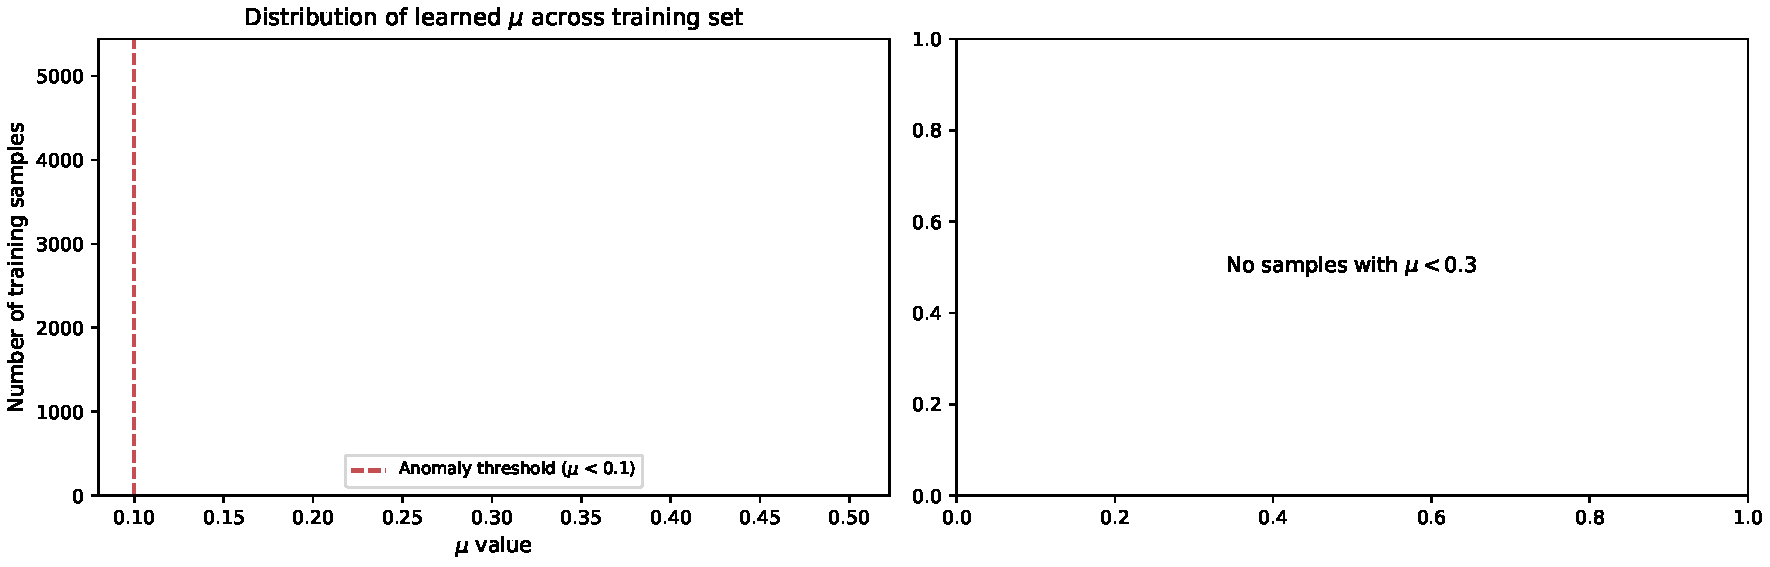
\includegraphics[width=\linewidth]{../figures/diagnostics/prae_mu_distribution_2015.pdf}\\
        {\tiny 2015: $\mu_i$ cluster at $0.502 \pm 0.0005$}
    \end{column}
    \begin{column}{0.48\textwidth}
        \centering
        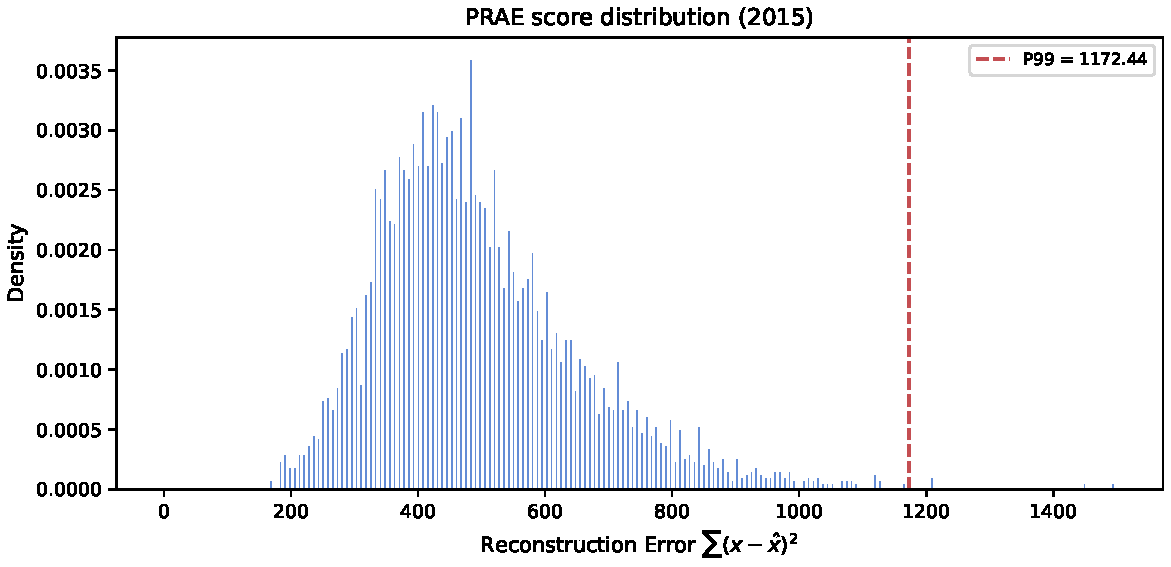
\includegraphics[width=\linewidth]{../figures/diagnostics/prae_score_distribution_2015.pdf}\\
        {\tiny 2015: reconstruction error distribution}
    \end{column}
    \end{columns}
    \vspace{0.2cm}
    \begin{itemize}
        \item Gate collapse: $\mu_i \approx 0.502$ both periods ($\text{std} < 0.001$)
        \item No rejection; behaves as standard autoencoder
        \item Lower 2017 $\lambda$: stronger outlier pressure, requires larger deviations to flag
        \item Compression yields more conservative 2017 scores
    \end{itemize}
    \note{Both models reduce to standard autoencoders. The $\ell_1$ regularisation weight and noise level $\sigma = 0.5$ are insufficient to force the gate to discriminate. Gate collapse is identical in both years: 2015 concentrates all 61{,}877 training $\mu_i$ at $0.502 \pm 0.0005$; 2017 concentrates 15{,}079 values at $0.502 \pm 0.0004$.}
\end{frame}


% ######################################################################
% SECTION 4: ANOMALY DETECTION RESULTS
% ######################################################################
\subsection{Anomaly Detection Results}

% ======================================================================
% SLIDE 15: ANOMALY RATES BY PERIOD
% ======================================================================
\begin{frame}{Anomaly Rates by Model and Intraday Period}
    \begin{columns}[T]
    \begin{column}{0.48\textwidth}
        \centering
        \includegraphics[width=\linewidth]{../figures/results/anomaly_rates_by_period_2015.pdf}\\
        {\tiny 2015-trained models}
    \end{column}
    \begin{column}{0.48\textwidth}
        \centering
        \includegraphics[width=\linewidth]{../figures/results/anomaly_rates_by_period_2017.pdf}\\
        {\tiny 2017-trained models}
    \end{column}
    \end{columns}
    \vspace{0.15cm}
    \begin{itemize}
        \item 2015 inter-model spread: PNN high, PRAE mid. 2017 TF-OCSVM anomaly rate near zero
        \item Models respond to different signals, not a common definition of anomaly
        \item US open elevation across years and models
        \item Intraday pattern stable across $\mathcal{T}_A$, $\mathcal{T}_B$
    \end{itemize}
    \note{Full anomaly rates: TF-OCSVM 2.0 to 2.8\% (2015) vs 0.00 to 0.03\% (2017), PNN 6.1 to 7.7\% vs 0.06 to 0.08\%, PRAE 2.2 to 3.7\% vs 2.1 to 2.5\%. The large gap for TF-OCSVM and PNN reflects a liberal $\tau_{2015}$ and narrow predicted $\sigma_{2015}$. The 2017 TF-OCSVM produces zero anomalies during the US open, suggesting its boundary is more conservatively calibrated for that regime.}
\end{frame}

% ======================================================================
% SLIDE 16: SCORE DISTRIBUTIONS
% ======================================================================
\begin{frame}{Score Distributions by Year}
    \begin{columns}[T]
    \begin{column}{0.48\textwidth}
        \centering
        \includegraphics[width=\linewidth]{../figures/results/score_distributions_2015.pdf}\\
        {\tiny 2015 score distributions}
    \end{column}
    \begin{column}{0.48\textwidth}
        \centering
        \includegraphics[width=\linewidth]{../figures/results/score_distributions_2017.pdf}\\
        {\tiny 2017 score distributions}
    \end{column}
    \end{columns}
    \vspace{0.15cm}
    \begin{itemize}
        \item 2017 TF-OCSVM range three-times narrower (longer training)
        \item Absolute thresholds non-transferable across years
        \item 2015 TF-OCSVM distribution has more borderline mass (2017 cleaner separation between normal and anomalous)
        \item PRAE right-skew remains stable across years
    \end{itemize}
    \begin{tcolorbox}[keybox, title=]
        Score scales differ by 1 to 2 orders; thresholds non-transferable.
    \end{tcolorbox}
    \note{TF-OCSVM 2015 spans $[-0.42, 0.13]$, 0.96\% cross zero; 2017 concentrated $[-0.12, 0.02]$, 0.025\% cross zero. PRAE mean reconstruction: 426.4 (2015) vs.\ 443.7 (2017). The compression of the 2017 score range is consistent with the OC-SVM learning a more representative normal boundary from more training data.}
\end{frame}

% ======================================================================
% SLIDE 17: MODEL AGREEMENT (CONSENSUS)
% ======================================================================
\begin{frame}{Model Agreement: Consensus Detection}
    \begin{columns}[T]
    \begin{column}{0.50\textwidth}
        \textbf{Consensus set:} 46{,}609 windows flagged by all three models in 2015 (0.04\% of total), \textbf{zero} in 2017.
        \vspace{0.1cm}
        \begin{itemize}
            \item 2017 two-model agreements mostly PRAE plus one
            \item Majority vote ($\geq 2$ models): 2015 huge, 2017 minimal
            \item Near-zero consensus: no shared anomaly definition
        \end{itemize}
    \end{column}
    \begin{column}{0.48\textwidth}
        \centering
        \includegraphics[width=\linewidth]{../figures/results/consensus_agreement_2015.pdf}\\[4pt]
        \includegraphics[width=\linewidth]{../figures/results/consensus_agreement_2017.pdf}
    \end{column}
    \end{columns}
    \note{Under the 2015 model: 89.56\% unanimously normal, 9.59\% flagged by one, 0.80\% by two, 0.04\% by all three. Under 2017: 97.74\% normal, 2.25\% by one, 0.005\% by two, 0\% by all three. The 2017 absence of full consensus is driven by the 150-fold reduction in PNN flag rate.}
\end{frame}

% ======================================================================
% SLIDE 18: THRESHOLD COMPARISON
% ======================================================================
\begin{frame}{Threshold Method Comparison}
    \centering
    \includegraphics[width=0.75\linewidth]{../figures/results/fig_5_3_jaccard_heatmaps.pdf}
    \vspace{0.1cm}

    Mean pairwise method agreement (CV of $\tau$): 0.67 (TF-OC-SVM), degenerate (PNN, DSPOT flags 99.8\%), 0.40 (PRAE).
    \vspace{0.1cm}
    \begin{itemize}
        \item PRAE inter-method agreement highest, robust to threshold choice
        \item TF-OCSVM sensitive to threshold method
        \item DSPOT invalid on bounded PNN scores
    \end{itemize}
    \note{Explicit thresholds: TF-OCSVM POT $\tau = 0.044$ (0.1\%), SPOT 0.018 (0.4\%), DSPOT 0.001 (0.9\%), RFDR 0.035 (0.2\%); PNN DSPOT drift correction drives $\tau$ to $-0.005$, flagging 99.8\%; PRAE POT $\tau = 3371$ (0.3\%), RFDR 1659 (0.5\%), SPOT/DSPOT ${\sim}1500$ (0.7\%). RFDR and POT are the most stable label-free methods across all three score streams.}
\end{frame}


% ######################################################################
% SECTION 5: PROXIMITY ANALYSIS
% ######################################################################
\section{Analysis}
\subsection{Proximity Analysis}

% ======================================================================
% SLIDE 19: PROXIMITY ANALYSIS
% ======================================================================
\begin{frame}{Proximity Effect: $\mathcal{T}_A$ vs.\ $\mathcal{T}_B$}
    \centering
    \includegraphics[width=0.75\linewidth]{../figures/results/fig_5_4_ta_vs_tb_dots.pdf}
    \vspace{0.1cm}
    \begin{table}[h]
    \centering
    \footnotesize
    \begin{tabular}{llrrl}
    \toprule
    \textbf{Model} & \textbf{Year} & $\bar{r}_A$ (\%) & $\bar{r}_B$ (\%) & $p$ \\
    \midrule
    TF-OCSVM & 2015 & 2.654 & 0.726 & 0.174 \\
    PNN      & 2015 & 2.598 & 4.010 & 0.100 \\
    PRAE     & 2015 & 3.624 & 3.713 & 0.812 \\
    TF-OCSVM & 2017 & 0.557 & 0.514 & 0.639 \\
    PNN      & 2017 & 0.008 & 0.012 & 0.597 \\
    \textbf{PRAE} & \textbf{2017} & \textbf{1.367} & \textbf{1.037} & \textbf{0.014} \\
    \bottomrule
    \end{tabular}
    \end{table}
    \begin{tcolorbox}[keybox, title=]
        Only 2017 PRAE shows a significant proximity effect.
    \end{tcolorbox}
    \note{The absence of a consistent proximity effect across models and years supports the validity of the test split design. The PRAE 2017 result is marginal and may reflect the longer training period rather than memorisation. Independent verification: under all four threshold methods (POT, SPOT, DSPOT, RFDR), PRAE shows $\mathcal{T}_A \gg \mathcal{T}_B$ (rates 2.3 to 2.5\% vs 0.01 to 0.04\%, 50 to 150$\times$), confirming this is a distributional property, not a threshold artefact.}
\end{frame}


% ######################################################################
% SECTION 6: SPOOFING GAIN ANALYSIS
% ######################################################################
\subsection{Spoofing Gain Analysis}

% ======================================================================
% SLIDE 20: GAIN DISTRIBUTIONS
% ======================================================================
\begin{frame}{Spoofing Gain Distribution}
    \centering
    \includegraphics[width=0.78\linewidth]{../figures/results/fig_5_5_gain_distribution.pdf}
    \vspace{0.15cm}
    \begin{itemize}
        \item 2015 gains degenerate: 90.6\% exactly zero
        \item 2017 left tail heavy, 0.07\% positive gains
    \end{itemize}
    \begin{tcolorbox}[keybox, title=]
        2017 positive gains: 0.07\%; interpretation remains open (unprofitability, model limitations, regulatory deterrence).
    \end{tcolorbox}
    \note{The near-zero gains in 2015 reflect the narrow predicted $\sigma$, which makes the fill probabilities near-degenerate. The 2017 distribution is better calibrated and produces meaningful gain estimates. The low positive-gain rate should not be interpreted as evidence that spoofing does not occur on TOTF.PA, only that the PNN framework does not identify it as profitable under the assumed fee structure. The batch gain computation uses a single PNN forward pass (Level-2 data limitation); the counterfactual feature vector is not recomputed, yielding a conservative estimate that neglects the distributional shift induced by the spoof order in Hawkes features.}
\end{frame}

% ======================================================================
% SLIDE 21: GAIN-SCORE ALIGNMENT
% ======================================================================
\begin{frame}{Gain-Score Alignment: Spearman Correlation}
    \centering
    \includegraphics[width=0.6\linewidth]{../figures/results/fig_5_5_gain_vs_score.pdf}
    \begin{table}[h]
    \centering
    \footnotesize
    \begin{tabular}{llrl}
    \toprule
    \textbf{Model} & \textbf{Year} & $\rho_s$ & \textbf{Interpretation} \\
    \midrule
    PNN      & both  & 1.000 & Tautological \\
    TF-OCSVM & 2017  & 0.415 & Flags less-costly-to-spoof states \\
    PRAE     & 2017  & $-0.143$ & Flags less spoofable states \\
    \bottomrule
    \end{tabular}
    \end{table}
    \begin{tcolorbox}[keybox, title=]
        TF-OCSVM scores align with spoofing, an emergent property.
    \end{tcolorbox}
    \note{The positive correlation for TF-OCSVM suggests that the latent representation captures book states that are structurally similar to those exploitable by spoofing, even though the model was trained only on reconstruction error. Score-decile analysis: mean $G$ increases monotonically from D1 (lowest) to D10 (highest) for TF-OCSVM in 2017. For PRAE, the trend reverses. On 2015, both correlations are negligible ($|\rho_s| < 0.06$) because $G$ is effectively constant at zero.}
\end{frame}

% ======================================================================
% SLIDE 22: FLAGGED VS NON-FLAGGED GAIN
% ======================================================================
\begin{frame}{Flagged vs.\ Non-Flagged Gain Distributions}
    \begin{columns}[T]
    \begin{column}{0.46\textwidth}
        \begin{itemize}
            \item TF-OCSVM flags less-negative gain states
            \item PRAE flags more-negative gain states
            \item Opposite gain direction across models
        \end{itemize}
    \end{column}
    \begin{column}{0.52\textwidth}
        \centering
        \includegraphics[width=\linewidth]{../figures/results/fig_5_5_gain_flagged_kde.pdf}
    \end{column}
    \end{columns}
    \begin{tcolorbox}[keybox, title=]
        TF-OCSVM flagged windows have 48\% higher (less negative) gain than non-flagged; PRAE flags the opposite direction.
    \end{tcolorbox}
    \note{The divergent relationship between reconstruction-based anomalies (PRAE) and density-based anomalies (TF-OCSVM) with respect to spoofing gain confirms that the models capture fundamentally different aspects of the anomaly landscape.}
\end{frame}


% ######################################################################
% SECTION 7: FEATURE ATTRIBUTION
% ######################################################################
\subsection{Feature Attribution}

% ======================================================================
% SLIDE 23: CROSS-MODEL HEATMAP
% ======================================================================
\begin{frame}{Cross-Model Feature Importance Heatmap}
    \centering
    \begin{columns}[T]
    \begin{column}{0.48\textwidth}
        \centering
        \includegraphics[width=\linewidth]{../figures/results/fig_5_6_cross_model_heatmap.pdf}
    \end{column}
    \begin{column}{0.48\textwidth}
        \centering
        \includegraphics[width=0.8\linewidth]{../figures/results/fig_5_6_occlusion_tf_ocsvm.pdf}
    \end{column}
    \end{columns}
    \vspace{0.1cm}
    \begin{itemize}
        \item Hawkes limit memory dominates PNN and PRAE
        \item Cancellation and return groups lead TF-OCSVM
        \item Trade-size importance strongest in 2015
    \end{itemize}
    \begin{tcolorbox}[keybox, title=]
        Top drivers across models: Hawkes limit-order memory and cancellation rapidity. Consistent with spoofing/layering signatures.
    \end{tcolorbox}
    \note{Methods: Integrated Gradients ($m{=}30$ steps) for PNN and PRAE, Grouped Occlusion for TF-OCSVM. Attribution computed on $n{=}150$ flagged windows per model per year. IG target: PNN $\to$ predicted scale $\sigma(\mathbf{x})$; PRAE $\to$ reconstruction error. Root-cause z-score analysis (independent of IG): TF-OCSVM top feature = Hawkes $M_{\text{bid}}$ ($\beta_{10}$) in 2015, $M_{\text{ask}}$ ($\beta_{1000}$) in 2017; PNN top = trade size (bid) in 2015, Hawkes $L_{\text{bid}}$ (short) in 2017.}
\end{frame}

% ======================================================================
% SLIDE 24: PNN ATTRIBUTION VARIANCE
% ======================================================================
\begin{frame}{PNN Feature Attribution: Consistent vs.\ Situational}
    \centering
    \includegraphics[width=0.7\linewidth]{../figures/results/fig_5_6_ig_variance_pnn.pdf}
    \vspace{0.15cm}
    \begin{itemize}
        \item 2015 top feature: \texttt{abs\_velocity} dynamics
        \item 2017 top-10: all Hawkes limit kernels
        \item Situational features (high variance): spread, OFI deep levels
        \item Consistent features (low variance): short half-life Hawkes limits
    \end{itemize}
    \begin{tcolorbox}[keybox, title=]
        Hawkes limit-order features are consistently ranked highest; dynamics features are year-specific and situational.
    \end{tcolorbox}
    \note{The year-specific shift from dynamics to Hawkes features reflects the change in volatility regime. On 2015 data (low $\sigma$), absolute velocity dominates because the PNN threshold is near-degenerate; on 2017 data, Hawkes features drive the calibrated gain calculation.}
\end{frame}

% ======================================================================
% SLIDE 25: CROSS-MODEL CONSENSUS FEATURES
% ======================================================================
\begin{frame}{Cross-Model Consensus: Top Feature Groups}
    Top groups across all three models (2017):
    \begin{itemize}
        \item Hawkes memory: placement intensity and distance
        \item Cancellation rapidity and size: spoofing withdrawal and quote stuffing
        \item Trade size and event flow: execution phase
        \item Lifecycle mapping: placement, shift, execution, cancellation
    \end{itemize}
    \begin{tcolorbox}[keybox, title=]
        All three models converge on features that trace the full spoofing lifecycle: placement, execution, cancellation.
    \end{tcolorbox}
    \note{The alignment between independently trained models on the same discriminative features provides indirect validation that the detected anomalies share structural properties with known spoofing signatures.}
\end{frame}


% ######################################################################
% SECTION 8: ANOMALY CLUSTERING
% ######################################################################
\subsection{Anomaly Clustering}

% ======================================================================
% SLIDE 26: CLUSTER PROJECTIONS
% ======================================================================
\begin{frame}{HDBSCAN Cluster Projections}
    \begin{columns}[T]
    \begin{column}{0.46\textwidth}
        \begin{itemize}
            \item 2015 anomalies: 1.34M, two clusters
            \item 2017 anomalies: 83K, two clusters
            \item 2017 separation stronger: silhouette +57\%
        \end{itemize}
        \begin{tcolorbox}[keybox, title=]
            HDBSCAN identifies two anomaly types in both years, with substantially better separation in 2017.
        \end{tcolorbox}
    \end{column}
    \begin{column}{0.52\textwidth}
        \centering
        \includegraphics[width=\linewidth]{../figures/results/fig_5_7_cluster_pca.pdf}
    \end{column}
    \end{columns}
    \note{Input to HDBSCAN: the three normalised anomaly scores per window. The two-cluster solution emerges consistently across years, suggesting a fundamental dichotomy in the anomaly landscape.}
\end{frame}

% ======================================================================
% SLIDE 27: CLUSTER FEATURE PROFILES
% ======================================================================
\begin{frame}{Cluster Feature Group Profiles}
    \begin{table}[h]
    \centering
    \footnotesize
    \begin{tabular}{lrrrl}
    \toprule
    \textbf{Year} & \textbf{Cluster} & \textbf{Size} & \textbf{Mean $G$} & \textbf{Profile} \\
    \midrule
    2015 & C0 & 1.29M (96\%) & $-0.8$  & Elevated imbalance + mid-price \\
    2015 & C1 & 39K (3\%)    & $-25.5$ & Depressed imbalance, elevated volatility \\
    2017 & C0 & 55K (66\%)   & $-54.4$ & PRAE-driven; elevated mid-price \\
    2017 & C1 & 25K (30\%)   & $-57.9$ & OC-SVM-driven; depressed deep-order \\
    \bottomrule
    \end{tabular}
    \end{table}

    \begin{columns}[T]
        \begin{column}{0.48\textwidth}
            \begin{tcolorbox}[keybox, title=]
                C0 = imbalance / reconstruction anomalies; \\C1 = volatility / boundary anomalies with larger spoofing cost.
            \end{tcolorbox}
        \end{column}
        \begin{column}{0.48\textwidth}
            \centering
            \includegraphics[width=0.9\linewidth]{../figures/results/fig_5_7_feature_group_profile.pdf}
        \end{column}
    \end{columns}
        
    \note{Cluster-specific gain values suggest C1 anomalies occur in market states where spoofing would be more costly. Per-model detection rates: 2017 C0 = 99.4\% PRAE, 0\% OC-SVM; C1 = 100\% OC-SVM, 0\% PRAE (near-perfect model alignment). 2015 C0 = 42\% PNN + 51\% PRAE (joint activation); C1 = 97\% OC-SVM. Noise cluster in 2017 has extreme mean $G = -4{,}800.9$. The two-cluster solution emerges consistently but aligns with model identity rather than a continuum of anomaly severity.}
\end{frame}


% ######################################################################
% SECTION 9: JUMP ANALYSIS
% ######################################################################
\subsection{Jump Analysis}

% ======================================================================
% SLIDE 28: JUMP CO-OCCURRENCE
% ======================================================================
\begin{frame}{Anomaly-Jump Co-Occurrence Rates}
    \begin{table}[h]
    \centering
    \footnotesize
    \begin{tabular}{llrrrl}
    \toprule
    \textbf{Year} & \textbf{Model} & \textbf{Rate} & \textbf{Base} & \textbf{Ratio} & $p$ \\
    \midrule
    2015 & TF-OCSVM & 16.10\% & 2.40\% & 6.7$\times$ & $< 5 \times 10^{-4}$ \\
    2015 & PNN      & 0.93\%  & 2.40\% & 0.4$\times$ & 1.000 \\
    2015 & PRAE     & 4.39\%  & 2.40\% & 1.8$\times$ & $< 5 \times 10^{-4}$ \\
    2017 & TF-OCSVM & 0.37\%  & 0.93\% & 0.4$\times$ & 1.000 \\
    2017 & PNN      & 17.09\% & 0.93\% & 18.4$\times$ & $< 5 \times 10^{-4}$ \\
    2017 & PRAE     & 11.39\% & 0.93\% & 12.3$\times$ & $< 5 \times 10^{-4}$ \\
    \bottomrule
    \end{tabular}
    \end{table}

    \begin{columns}[T]
        \begin{column}{0.55\textwidth}
            \begin{tcolorbox}[keybox, title=]
                Year-specific complementarity: TF-OCSVM detects jump-associated anomalies in 2015 but not 2017; PNN detects them in 2017 but not 2015. PRAE is the only model with elevated co-occurrence in both years.
            \end{tcolorbox}
        \end{column}
        \begin{column}{0.44\textwidth}
            \centering
            \includegraphics[width=0.8\linewidth]{../figures/results/fig_5_8_cooccurrence.pdf}
        \end{column}
    \end{columns}

    \note{Jump: absolute log-return $> 99.95$th percentile; horizon $\Delta t = 100$ events; permutation test with 2{,}000 shuffles. PNN in 2015 falls \emph{below} the base rate (0.93\% vs 2.40\%): its flags correspond to stable, non-jumping periods. TF-OCSVM in 2017 likewise falls below (0.37\% vs 0.93\%). Consensus set (2015 only, 7{,}044 windows): 3.65\% co-occurrence (1.5$\times$ base rate), diluted by anti-correlated PNN flags. No 2017 consensus exists.}
\end{frame}

% ======================================================================
% SLIDE 29: EVENT STUDY
% ======================================================================
\begin{frame}{Event Study: Price Path Around Flagged Windows}
    \begin{columns}[T]
        \begin{column}{0.48\textwidth}
            \begin{itemize}
                \item 2015 median lead time: 31 events
                \item 2017 median lead time: 6 events
                \item Flagged windows precede jumps above chance
            \end{itemize}
            \begin{tcolorbox}[keybox, title=]
                Anomalies precede jumps by median 6 to 31 events.
            \end{tcolorbox}
        \end{column}
        \begin{column}{0.48\textwidth}
            \centering
            \includegraphics[width=0.9\linewidth]{../figures/results/fig_5_8_price_path.pdf}
        \end{column}
    \end{columns}

    \note{The shorter lead time in 2017 may reflect a tighter OC-SVM boundary and more precise temporal localisation. The price path shape is consistent with the spoofing lifecycle: brief price displacement followed by partial reversion. At the aggregate level, the mean flagged price path is flat (buy and sell anomalies cancel), but the confidence band is wider than the non-flagged reference, confirming elevated local volatility around flagged windows.}
\end{frame}


% ######################################################################
% SECTION 10: CROSS-YEAR ROBUSTNESS
% ######################################################################
\subsection{Cross-Year Robustness}

% ======================================================================
% SLIDE 30: CROSS-YEAR ANOMALY RATES
% ======================================================================
\begin{frame}{Cross-Year Anomaly Rate Comparison}
    \begin{table}[h]
    \centering
    \footnotesize
    \begin{tabular}{llrrr}
    \toprule
    \textbf{Train} & \textbf{Model} & \textbf{In-year (\%)} & \textbf{Cross-year (\%)} & \textbf{Ratio} \\
    \midrule
    2015 & TF-OCSVM & 1.56 & 3.94  & 2.5$\times$ \\
    2015 & PNN      & 3.16 & 13.45 & 4.3$\times$ \\
    2015 & PRAE     & 3.84 & 2.02  & 0.5$\times$ \\
    2017 & TF-OCSVM & 0.56 & 0.00  & 0.0$\times$ \\
    2017 & PNN      & 0.01 & 0.05  & 6.2$\times$ \\
    2017 & PRAE     & 1.28 & 2.34  & 1.8$\times$ \\
    \bottomrule
    \end{tabular}
    \end{table}

    \begin{columns}[T]
        \begin{column}{0.48\textwidth}
            \begin{tcolorbox}[keybox, title=]
                PRAE is the most robust model. TF-OCSVM 2017 collapses entirely on 2015 data.
            \end{tcolorbox}
        \end{column}
        \begin{column}{0.48\textwidth}
            \centering
            \includegraphics[width=1.1\linewidth]{../figures/results/fig_5_9_anomaly_rate.pdf}
        \end{column}
    \end{columns}

    \note{The PNN trained on 2015 inflates to 13.45\% on 2017 data because the narrow $\sigma$ produces positive spoofing gains even for moderately large price moves characteristic of the 2017 volatility regime.}
\end{frame}

% ======================================================================
% SLIDE 31: DETECTION OVERLAP
% ======================================================================
\begin{frame}{Cross-Year Detection Set Overlap}
    \centering
    \includegraphics[width=0.7\linewidth]{../figures/results/fig_5_9_detection_overlap.pdf}

    \begin{columns}[T]
        \begin{column}{0.48\textwidth}
            \begin{itemize}
                \item PRAE overlap highest: $J = 0.18$
                \item TF-OCSVM and PNN overlaps near zero
            \end{itemize}
            \begin{tcolorbox}[keybox, title=]
                PRAE generalises best.
            \end{tcolorbox}
        \end{column}
        \begin{column}{0.48\textwidth}
            \begin{table}[h]
            \centering
            \footnotesize
            \begin{tabular}{llr}
            \toprule
            \textbf{Train} & \textbf{Model} & \textbf{Jaccard $J$} \\
            \midrule
            2015 & PRAE     & 0.073 \\
            2017 & PRAE     & 0.180 \\
            both & TF-OCSVM & $\approx 0$ \\
            both & PNN      & $\approx 0$ \\
            \bottomrule
            \end{tabular}
            \end{table}
        \end{column}
    \end{columns}

    \note{Jaccard $J = 0.18$ means that 18\% of the windows flagged by either the 2015- or 2017-trained PRAE are flagged by both, a non-trivial overlap for models trained 2 years apart on the same instrument.}
\end{frame}


% ######################################################################
% SECTION 11: DISCUSSION
% ######################################################################
\section{Discussion and Conclusion}
\subsection{Discussion}

% ======================================================================
% SLIDE 32: LIMITATIONS
% ======================================================================
\begin{frame}{Limitations}
    \begin{itemize}
        \item No ground-truth labels, precision and recall unavailable
        \item Single instrument (TOTF.PA), only three distal days per split
        \item Approximation and tail assumptions unquantified
        \item First-hour training misses intraday regime shifts
    \end{itemize}
    \note{The most consequential limitation is the absence of labels, which prevents reporting standard classification metrics and forces all evaluation to rely on indirect proxies (gain alignment, jump co-occurrence, cross-year overlap).}
\end{frame}

% ======================================================================
% SLIDE 33: COMPARISON OF APPROACHES
% ======================================================================
\begin{frame}{Comparison of Detection Approaches}
    \begin{table}[h]
    \centering
    \footnotesize
    \begin{tabular}{lp{2.5cm}p{2.5cm}p{2.5cm}}
    \toprule
    & \textbf{TF-OCSVM} & \textbf{PNN} & \textbf{PRAE} \\
    \midrule
    Score type     & Dissimilarity       & Spoofing gain $G$    & Reconstruction $\|x - \hat{x}\|^2$ \\
    $\rho_s$ with $G$ & +0.415 (2017)    & +1.000 (by design)  & $-0.143$ (2017) \\
    Jump co-occ.   & 6.7$\times$ (2015)   & 18.4$\times$ (2017) & Both years \\
    Cross-year $J$ & $\approx 0$          & $\approx 0$          & 0.07 to 0.18 \\
    Key drivers    & Cancellation         & Hawkes limit         & Hawkes limit \\
    \bottomrule
    \end{tabular}
    \end{table}
    \vspace{0.15cm}
    \begin{itemize}
        \item PNN interpretable, highly year-sensitive rates
        \item TF-OCSVM gain-aligned, weak cross-year transfer
        \item PRAE robust, lower spoofability alignment
        \item Deployment: PRAE+RFDR baseline, PNN for interpretability, periodic recalibration
    \end{itemize}
    \note{No single model dominates. A production system should combine PRAE for robustness with PNN for economic interpretability, using RFDR thresholding. PNN and TF-OCSVM require high-frequency retraining due to score-scale drift across years. The PRAE paired with dynamic relative thresholding represents the most stable single-model architecture for continuous deployment.}
\end{frame}

% ======================================================================
% SLIDE 34: INTERPRETATION
% ======================================================================
\begin{frame}{Interpretation: Detected Anomalies and Model Blind Spots}
    \begin{itemize}
        \item Spoofing signatures: Hawkes memory, rapid cancellations
        \item Legitimate overlap: volume surges, spread expansions
        \item Blind spot: subtle low-volume spoofing
        \item Blind spots: multi-day and message-rate manipulation
    \end{itemize}
    \begin{tcolorbox}[keybox, title=]
        Definitive classification requires regulatory cross-referencing; the pipeline identifies candidate events with structural spoofing properties.
    \end{tcolorbox}
    \note{The two-cluster taxonomy from HDBSCAN partially separates the spoofing-type pattern from the volume-type pattern. Full disambiguation requires order-level (Level-3) data.}
\end{frame}


% ######################################################################
% SECTION 12: CONCLUSION
% ######################################################################
\subsection{Conclusion}

% ======================================================================
% SLIDE 35: CONTRIBUTIONS
% ======================================================================
\begin{frame}{Contributions}
    \begin{itemize}
        \item Three-model unsupervised pipeline on equity LOB
        \item 89-feature library, Hawkes and cancellation drivers
        \item Equity spoofing-gain application: 0.07\% positive windows
        \item Threshold and robustness ranking, PRAE strongest
    \end{itemize}
    \note{The main finding is that unsupervised probabilistic models can detect structurally consistent anomalies across years, but each model captures a different anomaly facet. The PRAE is the recommended single-model choice for robustness.}
\end{frame}

% ======================================================================
% SLIDE 36: FUTURE WORK
% ======================================================================
\begin{frame}{Future Work}
    \begin{itemize}
        \item Multi-asset evaluation across venues and classes
        \item Level-3 integration for intent-level classification
        \item Richer density models and continual learning (e.g., attention-based architecture for PNN)
        \item Crypto validation and synthetic spoofing calibration
    \end{itemize}
    \note{The most impactful next step is cryptocurrency validation, where the higher manipulation base rate provides a natural validation set for the pipeline's detection capabilities.}
\end{frame}


% ######################################################################
% CLOSING
% ######################################################################
\begin{frame}{}
    \centering
    \LARGE{Thank you for your attention.}
\end{frame}


% ######################################################################
% BIBLIOGRAPHY
% ######################################################################
\begin{frame}[allowframebreaks]
    \frametitle{Bibliography}
    \nocite{*}
    \printbibliography
\end{frame}


% ######################################################################
% APPENDIX
% ######################################################################
\appendix
\section{Appendix}

% ======================================================================
% APPENDIX A1: DAILY ANOMALY RATES
% ======================================================================
\begin{frame}{Appendix: Daily Anomaly Rates}
    \begin{columns}[T]
    \begin{column}{0.48\textwidth}
        \centering
        \includegraphics[width=\linewidth]{../figures/results/daily_anomaly_rates_2015.pdf}\\
        {\tiny 2015}
    \end{column}
    \begin{column}{0.48\textwidth}
        \centering
        \includegraphics[width=\linewidth]{../figures/results/daily_anomaly_rates_2017.pdf}\\
        {\tiny 2017}
    \end{column}
    \end{columns}
\end{frame}

% ======================================================================
% APPENDIX A2: SCORE TIME SERIES
% ======================================================================
\begin{frame}{Appendix: Anomaly Score Time Series}
    \begin{columns}[T]
    \begin{column}{0.48\textwidth}
        \centering
        \includegraphics[width=\linewidth]{../figures/results/score_timeseries_2015.pdf}\\
        {\tiny 2015}
    \end{column}
    \begin{column}{0.48\textwidth}
        \centering
        \includegraphics[width=\linewidth]{../figures/results/score_timeseries_2017.pdf}\\
        {\tiny 2017}
    \end{column}
    \end{columns}
\end{frame}

% ======================================================================
% APPENDIX A3: THRESHOLD VALUES
% ======================================================================
\begin{frame}{Appendix: Threshold Levels by Method and Model}
    \centering
    \includegraphics[width=0.82\linewidth]{../figures/results/fig_5_3_threshold_values.pdf}
\end{frame}

% ======================================================================
% APPENDIX A4: ROOT-CAUSE FEATURES
% ======================================================================
\begin{frame}{Appendix: Root-Cause Feature Rankings}
    \begin{columns}[T]
    \begin{column}{0.48\textwidth}
        \centering
        \includegraphics[width=\linewidth]{../figures/results/root_cause_features_2015.pdf}\\
        {\tiny 2015}
    \end{column}
    \begin{column}{0.48\textwidth}
        \centering
        \includegraphics[width=\linewidth]{../figures/results/root_cause_features_2017.pdf}\\
        {\tiny 2017}
    \end{column}
    \end{columns}
\end{frame}

% ======================================================================
% APPENDIX A5: IG BAR CHARTS
% ======================================================================
\begin{frame}{Appendix: Integrated Gradient Attribution}
    \begin{columns}[T]
    \begin{column}{0.48\textwidth}
        \centering
        \includegraphics[width=\linewidth]{../figures/results/fig_5_6_ig_bar_pnn.pdf}\\
        {\tiny PNN}
    \end{column}
    \begin{column}{0.48\textwidth}
        \centering
        \includegraphics[width=\linewidth]{../figures/results/fig_5_6_ig_bar_prae.pdf}\\
        {\tiny PRAE}
    \end{column}
    \end{columns}
\end{frame}

% ======================================================================
% APPENDIX A6: TF-OCSVM OCCLUSION
% ======================================================================
\begin{frame}{Appendix: TF-OCSVM Grouped Occlusion}
    \centering
    \includegraphics[width=0.82\linewidth]{../figures/results/fig_5_6_occlusion_tf_ocsvm.pdf}
\end{frame}

% ======================================================================
% APPENDIX A7: LEAD TIME
% ======================================================================
\begin{frame}{Appendix: Anomaly-Jump Lead Time Distribution}
    \centering
    \includegraphics[width=0.82\linewidth]{../figures/results/fig_5_8_lead_time.pdf}
\end{frame}

% ======================================================================
% APPENDIX A8: CLUSTER TEMPORAL
% ======================================================================
\begin{frame}{Appendix: Anomaly Cluster Temporal Distribution}
    \centering
    \includegraphics[width=0.82\linewidth]{../figures/results/fig_5_7_cluster_temporal.pdf}
\end{frame}

% ======================================================================
% APPENDIX A9: ARCHITECTURE DETAILS - TF-OCSVM
% ======================================================================
\begin{frame}{Appendix: Architecture Details - TF-OCSVM}
    \begin{tcolorbox}[keybox, title=Transformer Bottleneck AE]
        \begin{itemize}
            \item Input $(25 \times 89)$ $\to$ 128-dim latent $\to$ reconstruction
            \item 6 layers, 8 heads, $d_{\text{ff}}{=}512$; MSE loss (Adam, $\eta{=}10^{-4}$, patience 20)
            \item Gradient clipping: max norm 1.0
        \end{itemize}
    \end{tcolorbox}
    \begin{tcolorbox}[keybox, title=Nystr{\"o}m OC-SVM]
        \begin{itemize}
            \item Nystr{\"o}m approximation ($m{=}300$ landmarks), RBF $\gamma$ via median heuristic
            \item SGD training (500 epochs, $\nu{=}0.01$, lr $= 10^{-2}$, momentum 0.9, batch 256)
            \item Offset $\rho$ reset to $\nu$-quantile of training projections after SGD
        \end{itemize}
    \end{tcolorbox}
    \begin{tcolorbox}[keybox, title=Dissimilarity Score]
        $d(\mathbf{z}) = -f(\mathbf{z}) = \rho - \mathbf{w}^\top \Phi(\mathbf{z})$; \quad baseline $\tau_0 = Q_{1-\nu}$ of training scores
    \end{tcolorbox}
\end{frame}

% ======================================================================
% APPENDIX A10: ARCHITECTURE DETAILS: PNN
% ======================================================================
\begin{frame}{Appendix: Architecture Details: PNN}
    \begin{tcolorbox}[keybox, title=Architecture]
        \begin{itemize}
            \item Single hidden layer ($d_h{=}64$, ReLU), Markovian: last time step only
            \item Output: skew-normal parameters $(\mu, \sigma, \alpha)$ for $\Delta p_{\text{mid}}$
            \item $\sigma = \mathrm{Softplus}(\sigma_{\text{raw}}) + 10^{-6}$
        \end{itemize}
    \end{tcolorbox}
    \begin{tcolorbox}[keybox, title=Training Objective]
        Skew-normal NLL: $\mathcal{L} = -\frac{1}{|\mathcal{B}|}\sum_i \ln\bigl(\frac{2}{\sigma_i}\,\varphi(z_i)\,\Phi(\alpha_i z_i) + 10^{-10}\bigr)$
    \end{tcolorbox}
    \begin{tcolorbox}[keybox, title=Spoofing Gain Parameters]
        $Q{=}4{,}500$, $q{=}100$, $\delta_a{=}0$, $\delta_b{=}0.01$; maker fee $\varepsilon^+{=}0$, taker fee $\varepsilon^-{=}8 \times 10^{-4}$ (Euronext Paris)
    \end{tcolorbox}
\end{frame}

% ======================================================================
% APPENDIX A11: ARCHITECTURE DETAILS: PRAE
% ======================================================================
\begin{frame}{Appendix: Architecture Details: PRAE}
    \begin{tcolorbox}[keybox, title=Architecture]
        \begin{itemize}
            \item Same Transformer backbone as TF-OCSVM ($d_{\text{model}}{=}128$, $h{=}8$, $N{=}6$)
            \item Learnable per-sample gate: $g_i = \mathrm{clamp}(\mu_i + \varepsilon_i,\; 0,\; 1)$, \quad $\varepsilon_i \sim \mathcal{N}(0,\, 0.5^2)$
            \item Gate initialisation: $\mu_i = 0.5$; per-sample errors clamped to $10^6$
        \end{itemize}
    \end{tcolorbox}
    \begin{tcolorbox}[keybox, title=Training Objective]
        $\mathcal{L}_1 = \mathbb{E}\bigl(\sum_i g_i \|x_i - \hat{x}_i\|^2 - \lambda \|\mathbf{g}\|_1\bigr)$
    \end{tcolorbox}
    \begin{tcolorbox}[keybox, title=$\lambda$ Tuning (Day~1)]
        $\lambda_{\text{heuristic}} = \overline{\|\mathbf{x}\|^2} \cdot k \cdot d_{\text{in}}$; grid search over $\{0.001, 0.005, \ldots, 1.0\}$ multipliers, 15 epochs each. Result: $\lambda_{2015} = 1109.3$, $\lambda_{2017} = 215.4$.
    \end{tcolorbox}
\end{frame}

\end{document}
